\documentclass{tufte-handout}
\usepackage{../braph2_dev}
%\geometry{showframe} % display margins for debugging page layout

\title{General Developer Tutorial for BRAPH 2.0}

\author[The BRAPH~2 Developers]{The BRAPH~2 Developers}

\begin{document}

\maketitle

\begin{abstract}
\noindent
The software architecture of BRAPH~2.0 provides a clear structure for developers to understand and extend its functionalities. All objects (\emph{elements}) in BRAPH~2.0 are derived from the base object \code{Element}. Developers can easily add new elements by writing the new elements in the simplified BRAPH~2.0 pseudocode. 
By recompiling BRAPH~2.0, the new elements and their functionalities are immediately integrated, also into the graphical user interface.
In this Developer Tutorial, we will explain how BRAPH~2.0 is compiled, how the elements are strcutured, and how new elements can be implemented.
\end{abstract}

\tableofcontents

%%%%% %%%%% %%%%% %%%%% %%%%%
\clearpage
\section{Compilation and Element (Re)Generation}

BRAPH~2.0 is a compiled object-oriented programming software.
Its objects are \emph{elements}, which contain a set of \emph{props} of various \emph{categories} and \emph{formats}, as described in detail in the following sections. 
These elements are written in the BRAPH~2.0 pseudocode, which simplifies and streamlines the coding process.
To convert them into usable matlab objects, BRAPH~2.0 needs to be compiled, which is done by calling the script \code{braph2genesis}, which will compile the whole code, as shown in \Coderef{cd:compilation}.
%
\begin{lstlisting}[
	label=cd:compilation,
	caption={
		{\bf Compilation of BRAPH~2.0.}
		Executing the script \code{braph2genesis} compiles BRAPH~2.0 and , subsequently, unit tests it.
		Importantly, this function might take several hours to run (plus several more hours to unit test the compiled code).
	}
]
>> braph2genesis
\end{lstlisting}

During the compilation, there are several phases to improve the computational efficiency of the executable code:
\begin{enumerate}
	\item {\bf First compilation}, where the elements are created.
	\item {\bf Second compilation}, where the elements are computationally optimized.
	\item {\bf Constant hard-coding}, where several contants are hard-coded in the executable code to further optimize the run time.
\end{enumerate}

Because this multi-stage compilation, it is not always possible to regenerate a single element without regenerating the whole BRAPH~2.0. 
Nevertheless, it is usually possible to regenerate a single element as long as the element already exists and its props have not been changed.
This can be done with the function \code{regenerate()}, as shown in \Coderef{cd:regenerate}.
%
\begin{lstlisting}[
	label=cd:regenerate,
	caption={
		{\bf Regeneration of elements.}
		The function \code{regenerate()} can be used to regenerate some elements, as long as they already exist in the current BRAPH~2.0 compilation and their list of props has not been altered (e.g., renamed, moved, added). In this case, it is necessary to recompile BRAPH~2.0 with \code{braph2genesis}.
	}
]
>> close all; delete(findall(0, 'type', 'figure')); clear all ¥\circled{1}\circlednote{1}{clears the workspace (not always necessary, but needed is some element instances are still in the workspace).}¥

>> regenerate(regenerate('/src/gui', {'Pipeline'}) ¥\circled{2}\circlednote{2}{regenerates \code{Pipeline}.}¥

>> regenerate(regenerate('/src/gui', {'Pipeline'}, 'DoubleCompilation', false) ¥\circled{3}\circlednote{3}{performs only one compilation.}¥

>> regenerate(regenerate('/src/gui', {'Pipeline'}, 'CreateElement', false) ¥\circled{4}\circlednote{4}{does not regenerate the element, but only the layout and the unit test.}¥

>> regenerate(regenerate('/src/gui', {'Pipeline'}, 'CreateLayout', false) ¥\circled{5}\circlednote{5}{does not regenerate the layout.}¥

>> regenerate(regenerate('/src/gui', {'Pipeline'}, 'CreateTest', false) ¥\circled{6}\circlednote{6}{does not regenerate the unit test.}¥

>> regenerate(regenerate('/src/gui', {'Pipeline'}, 'UnitTest', false) ¥\circled{7}\circlednote{7}{does not perform the unit test.}¥

>> regenerate(regenerate('/src/gui', {'Pipeline'}, 'CreateLayout', false, 'UnitTest', false) ¥\circled{8}\circlednote{8}{Multiple options can be selected at once. In this ces, it does not regenerate the layout and it does not perform the unit test.}¥

>> regenerate(regenerate('/src/gui', {'Pipeline', 'GUI'}) ¥\circled{9}\circlednote{9}{Multiple elements can be regenerated at once. This can throw an error, typically because an instance of the element to be regenerated remains in the workspace. In this case, regenerate the elements one by one.}¥
\end{lstlisting}

\section{Elements}

The base class for all elements is \code{Element}. 
Each element is essentially a container for a series of \emph{props} (properties). Each prop is characterized by the following static features (i.e., equal for all instances of the prop):
\begin{itemize}
	\item A \emph{sequential number} (integer starting from 1).
		
	\item A \emph{tag} (a string).
	
	\item A \emph{category}, which determines for how a prop is used.\footnote{The possible categories and formats are shown in the boxes below.}
	
	\item A \emph{format}, which determines what a prop can contain.
\end{itemize}
The functions to inspect these features can be found by using the command \code{help Element} in the MatLab command line.

Furthermore, each instance of a prop has the following features:
\begin{itemize}
	\item A \emph{value}.\footnote{The value is by defalut a \code{NoValue}. For \code{PARAMETER}, \code{DATA}, \code{FIGURE}, and \code{GUI} props, it can also be a callback. For \code{CONSTANT} props, it is usually a concrete value.}
	The functions to set, get, and memorize a value will be discussed in the following sections.
	
	\item A \emph{seed} for the random number generator to ensure the reproducibility of the results. 
	The seed of each property is a 32-bit unsigned integer and is initialized when an element is constructed by calling \code{randi(intmax('uint32'))}.
	
	The seed can be obtained using:\\
	\code{seed = el.getPropSeed(pointer)}\\
	where \code{pointer} can be either a prop number or tag.
	It cannot be changed.
 	
	\item A \emph{checked} status, which is true by default.
	Checked props are checked for format when they are set and for value when they are set/calculated.\footnote{When \code{BRAPH2.CHECKED = false}, no checks are performed. This needs to be changes in the file \fn{BRAPH2.m}.}
	
	The checked status of a prop can be altered with the functions:\\
	\code{el.checked(pointer)}\\
	\code{el.unchecked(pointer)}\\
	The checked status of a prop can be assessed with the function:
	\code{checked = el.isChecked(pointer)}\\
	where \code{pointer} can be either a prop number or tag.
	
	\item A \emph{locked} status, which is false by default.\footnote{The \code{PARAMETER} and \code{DATA} props get locked the first time a \code{RESULT} property is successfully calculated. The locked status is not used for \code{CONSTANT} props.}
	
	A prop can be locked with the function:\\
	\code{el.lock(pointer)}\\
	Once locked, it cannot be unlocked.
	The locked status of a prop can be assessed with the function:\\
	\code{locked = el.isLocked(pointer)}\\
	where \code{pointer} can be either a prop number or tag.
	
	\item A \emph{callback} instance.\footnote{Callbacks are not used with \code{METADATA} props.}
	
	The callback to a prop can be obtained using the function:\\
	\code{cb = el.getCallback(pointer)}\\
	where \code{pointer} can be either a prop number or tag.
	
\end{itemize}
Additional functions to operate with these features can be found by using the command \code{help Element} in the MatLab command line.

\begin{fullwidth}
\begin{tcolorbox}[
	title=Property Categories
]
\begin{description} 
 	\item[\code{CONSTANT}] Static constant equal for all instances of the element. It allows incoming callbacks.
 
 	\item[\code{METADATA}] Metadata NOT used in the calculation of the results. It does not allow callbacks. It is not locked when a result is calculated.
 
 	\item[\code{PARAMETER}] Parameter used to calculate the results of the element. It allows incoming and outgoing callbacks. It is connected with a callback when using a template. It is locked when a result is calculated.
 
 	\item[\code{DATA}] Data used to calculate the results of the element. It is \code{NoValue} when not set. It allows incoming and outgoing callbacks. It is locked when a result is calculated.
 
 	\item[\code{RESULT}] Result calculated by the element using parameters and data. The calculation of a result locks the element. It is \code{NoValue} when not calculated. It allows incoming callbacks.
 
 	\item[\code{QUERY}] Query result calculated by the element. The calculation of a query does NOT lock the element. It is \code{NoValue} when not calculated. Typically, it should not be memorized.
It does not allow callbacks.
 
 	\item[\code{EVANESCENT}] Evanescent variable calculated at runtime (typically employed for handles of GUI components). It is \code{NoValue} when not calculated. Typically, it should be memorized at first use.
It does not allow callbacks.
 
 	\item[\code{FIGURE}] Parameter used to plot the results in a figure. It allows incoming and outgoing callbacks. It is not locked when a result is calculated.
                
 	\item[\code{GUI}] Parameter used by the graphical user interface (GUI). It allows incoming and outgoing callbacks. It is not locked when a result is calculated.
\end{description}
\end{tcolorbox}
\end{fullwidth}

\begin{fullwidth}
\begin{tcolorbox}[
	title=Property Categories
]
\begin{description} 
	\item [\code{EMPTY}] Empty has an empty value and is typically used as a result or query to execute some code. 
 
	\item [\code{STRING}] String is a char array.
 
	\item [\code{STRINGLIST}] StringList is a cell array with char arrays.
 
	\item [\code{LOGICAL}] Logical is a boolean value.
 
	\item [\code{OPTION}] Option is a char array representing an option within a set defined in the element (case sensitive).\\ 
                Settings: cell array of chars representing the options, e.g., \code{\{'plus', 'minus', 'zero'\}}.
 
	\item [\code{CLASS}] Class is a char array corresponding to an element class.\\
                Settings: class name of a subclass of Element (or Element itself).
 
	\item [\code{CLASSLIST}] ClassList is a cell array with char arrays corresponding to element classes.\\
                Settings: class name of a subclass of Element (or Element itself), which represents the base element.
 
	\item [\code{ITEM}] Item is a pointer to an element of a class defined in the element.\\ 
                Settings: class name of a subclass of Element (or Element itself).
 
	\item [\code{ITEMLIST}] ItemList is a cell array with pointers to elements of a class defined in the element.\\
                Settings: class name of a subclass of Element (or Element itself), which represents the base element.
 
	\item [\code{IDICT}] Idict is an indexed dictionary of elements of a class defined in the element.\\
                Settings: class name of a subclass of Element (or Element itself), which represents the dictionary element.
 
	\item [\code{SCALAR}] Scalar is a scalar numerical value.
 
	\item [\code{RVECTOR}] RVector is a numerical row vector.
 
	\item [\code{CVECTOR}] CVector is a numerical column vector.
 
	\item [\code{MATRIX}] Matrix is a numerical matrix.
 
	\item [\code{SMATRIX}] SMatrix is a numerical square matrix.
 
	\item [\code{CELL}] Cell is a 2D cell array of numeric data, typically used for adjaciency matrices and measures.
 
	\item [\code{NET}] Net is a MatLab neural network object (network, SeriesNetwork, DAGNetwork, dlnetwork).
 
	\item [\code{HANDLE}] Handle is a handle for a graphical or listener component. It should only be used as an evanescent property.
 
	\item [\code{HANDLELIST}] HandleList is a cell array with handles for graphical or listener components. It should only be used as an evanescent property.
 
	\item [\code{COLOR}] Color is an RGB color, e.g., \code{'[1 0 0]'} for red.
 
	\item [\code{ALPHA}] Alpha is a transparency level between 0 and 1.
 
	\item [\code{SIZE}] Size represents the size of a graphical componet. It is a positive number (default = 1).
 
	\item [\code{MARKER}] Marker represents the marker style.
                It can be \code{'o'}, \code{'+'}, \code{'*'}, \code{'.'}, 'x', \code{'\_'}, \code{'|'}, \code{'s'}, \code{'d'}, \code{'\^'}, \code{'v'}, \code{'>'}, \code{'<'}, \code{'p'}, \code{'h'}, \code{''} (no marker).
 
	\item [\code{LINE}] Line represents the line style. It can be \code{'-'}, \code{':'}, \code{'-.'}, \code{'--'}, \code{''} (no line).
\end{description}
\end{tcolorbox}
\end{fullwidth}

Even though it is possible to create instances of \code{Element}, typically one uses its subclasses and does not have any props.
Its three direct subclasses are \code{NoValue}, \code{Callback}, and \code{ConcreteElement}, as shown in \Figref{fig:elements}.

\fig{figure*}
	{fig:elements}
	{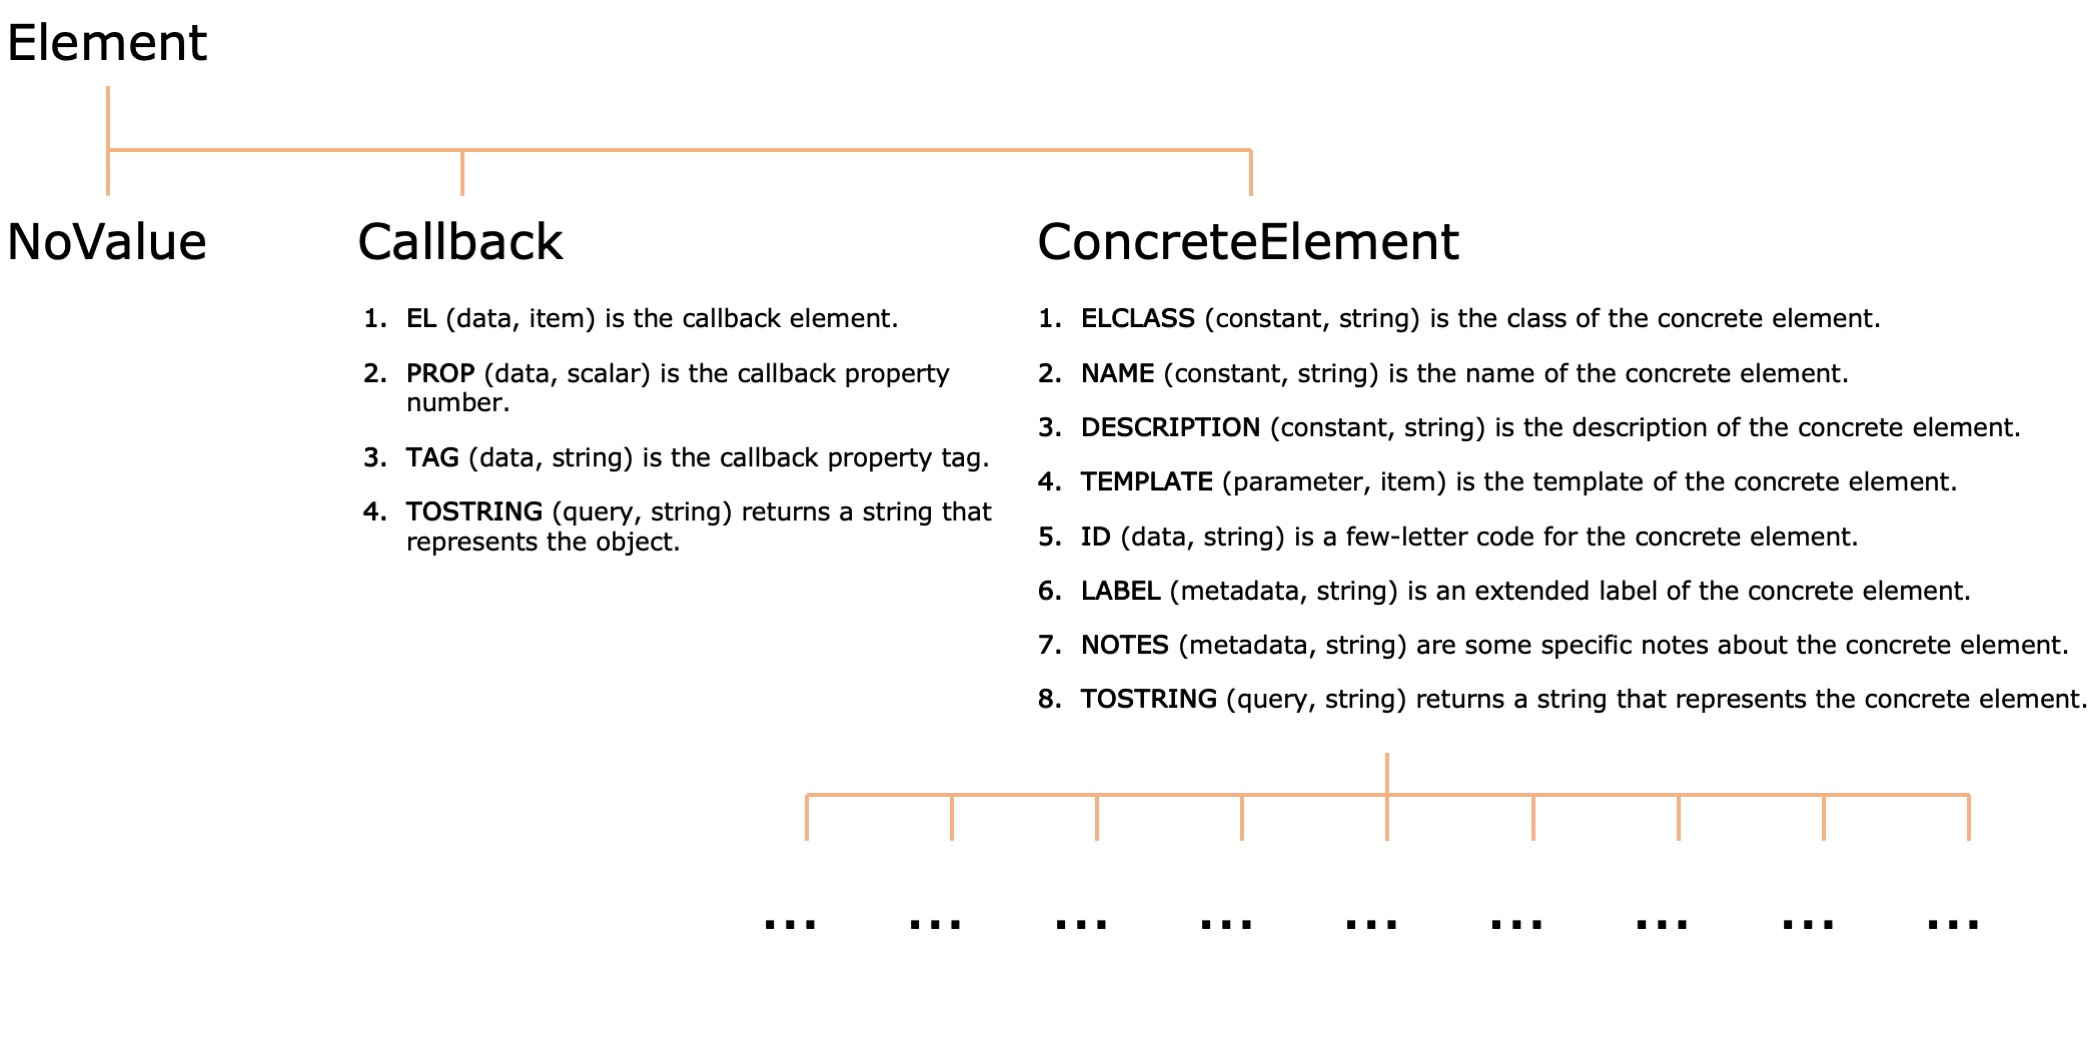
\includegraphics{fig01_big.jpg}}
	{Element tree}
	{
	All elements derive from the base class \code{Element}. 
	Its direct children are \code{NoValue}, \code{Callback}, and \code{ConcreteElement}, whose properties are also indicated.
	Concrete elements further derive directly or indirectly from \code{ConcreteElement}.
	}

The element \code{NoValue} is used to represent a value that has not been set (for properties of categories \code{METADATA}, \code{PARAMETER}, \code{DATA}, \code{FIGURE} or \code{GUI}) or calculated (for properties of category \code{RESULT}, \code{QUERY}, \code{EVANESCENT}), while it should not be used for properties of category \code{CONSTANT}.
It should be instantiated using \Coderef{cd:novalue}.
%
\begin{lstlisting}[
	label=cd:novalue,
	caption={
		{\bf Instantiation of \code{NoValue}.}
		For computational efficiency, it is best to use only one instance using this script, instead of creating new instances using the constructor \code{NoValue()}. 
	}
]
Element.getNoValue()
\end{lstlisting}
%
No element can be a subclass of NoValue.
  
A \code{Callback} refers to a prop of another element \code{el}, identified by prop number or tag.
It should be instantiated using \Coderef{cd:callback}.
%
\begin{lstlisting}[
	label=cd:callback,
	caption={
		{\bf Instantiation of a \code{Callback}.}
		For computational efficiency, it is best to use only one instance of \code{Callback} for each prop of an instance of a concrete element \code{el} with the code shown below, instead of creating new callback instances using its constructor. 
	}
]
el.getCallback('PROP', PROP_NUMBER)
el.getCallback('TAG', PROP_TAG)
\end{lstlisting}
%
No element can be a subclass of \code{Callback}.

A concrete element (\code{ConcreteElement}) provides the infrastructure necessary for all concrete elements. 
In particular, it has the constant props \code{ELCLASS} (string), \code{NAME} (string) and \code{DESCRIPTION} (string), the property \code{TEMPLATE} (item), the indexing properties \code{ID} (string), \code{LABEL} (string), and \code{NOTES} (string), and the query prop \code{TOSTRING} (string).
Even though it is possible to create instances of \code{ConcreteElement}, typically one uses its subclasses.

\subsection{Setting Props}

The value of a prop can be set with \Coderef{cd:set}.
%
\begin{lstlisting}[
	label=cd:set,
	caption={
		{\bf Setting a prop.}
		This script illustrates various ways in which props can be set.
	}
]
el.set('ID', 'new el id') ¥\circled{1}\twocirclednotes{1}{2}{set the value of a prop with the prop tag or the prop number.}¥
el.set(5, 'new el id') ¥\circled{2}¥

el.set( ... ¥\circled{3}\circlednote{3}{sets the values of multiple props at once. The pointers can be either property numbers or property tags.}¥
	'ID', 'new el id', ...
	'LABEL', 'new el label', ...
	7, 'new el notes' ...
	) 

el = el.set('ID', 'new el id') ¥\circled{3}\circlednote{3}{returns the element.}¥
\end{lstlisting}
%
When a prop is set to a certain value, the following operations are performed:
\begin{enumerate}
	\item The value is {\bf conditioned} before being set (by calling the protected \emph{static} function \code{conditioning()}, which can be defined in each subelement).
	
	This can be set with the token \code{¡conditioning!}.
	
	\item The value is {\bf preset} before being set (by calling the protected function \code{preset()}, which can be defined in each subelement).\footnote{Differently from the \emph{static} function \code{conditioning()}, the function \code{preset()} has access to the element instance.}

	This can be set with the token \code{¡preset!}.
	
	\item If a property is checked, its {\bf format is checked} before proceeding to its setting by calling \code{Format.checkFormat()}.\\
	If the check fails, the property is not set and an error is thrown with error id\\
	\code{BRAPH2:<Element Class>:WrongInput}.
	
	This can be set with the token \code{¡checkProp!}.

	\item The value is {\bf set}.

		If the property is of category \code{PARAMETER}, \code{DATA}, \code{FIGURE}, or \code{GUI}, the value is set only if the property is unlocked.\\
		If an attempt is made to set a locked property, no setting occurs and a warning is thrown with warning id \code{BRAPH2:<Element Class>}.\\
		If the value is a callback, a warning is thrown if the element, property number and/or settings of the callback do not coincide with those of the property with warning id\\
		\code{BRAPH2:<Element Class>}.
 
		If the property is of category RESULT, QUERY or EVANESCENT, the value can only be set to \code{Element.getNoValue()}.

	\item The value is {\bf postset} after being set (by calling the protected function \code{postset()}, which is defined in each subelement).
	
	This can be set with the token \code{¡postset!}.

	\item {\bf All props} are {\bf postprocessed} after being set (by calling the protected function \code{postprocessing()}, which is defined in each subelement).
	
	This can be set with the token \code{¡postprocessing!}.

	\item If ANY property is checked, the function \code{Element.check()} is called after all settings are made and the consistency of the values of {\bf all pros} are {\bf checked}.\\
	If the check fails an error is thrown with error id\\
	\code{BRAPH2:<Element Class>:WrongInput}.
	
	\item When a prop is successfully set, an {\bf event} \code{PropSet()} is {\bf notified}.
\end{enumerate} 

\subsection{Getting Props}

The value of a prop can be retrieved with \Coderef{cd:get}.
%
\begin{lstlisting}[
	label=cd:get,
	caption={
		{\bf Getting a prop.}
		This script illustrates various ways in which the value of a prop can be retrieved.
	}
]
value = el.get('ID'); ¥\circled{1}\circlednote{1}{gets the value of a prop using the prop tag.}¥

value = el.get(ConcreteElement.ID); ¥\circled{2}\circlednote{2}{gets the value of a prop using the prop number.}¥

el.get('ID') ¥\circled{3}\twocirclednotes{3}{4}{do not return any output value. This can be useful, e.g., when a code needs to be executed, e.g., by a \code{QUERY}.}¥
el.get(ConcreteElement.ID) ¥\circled{4}¥

value = el.get('QUERY', ARG1, ARG2, ... ); ¥\circled{5}\circlednote{5}{can be used with a series of arguments for props of category \code{QUERY}. Any additional arguments are ignored for props of other categories.}¥
\end{lstlisting}

If the raw value of the property is a \code{NoValue}, it proceed to return the default property value (for categories \code{METADATA}, \code{PARAMETER}, \code{DATA}, \code{FIGURE}, and \code{GUI}).
 
If the raw value of the property is a callback, it retrieves the value of the linked property (for categories \code{PARAMETER}, \code{DATA}, \code{FIGURE}, and \code{GUI}).
 
If a property of category \code{RESULT}, \code{QUERY}, or \code{EVANESCENT} is not calculated (i.e., its raw value is \code{NoValue}), it proceeds to calculate it (but not to memorize it, i.e., its raw value remains \code{NoValue}). After the calculation of a property of category \code{RESULT} all properties of categories \code{PARAMETER} and \code{DATA} are irreversibly locked.
If the property is checked, it proceeds to check all properties after the calculation calling the function \code{check()}. If the check fails, it resets the property to \code{NoValue} and returns \code{NoValue}, does not lock the property, and throws a warning with warning id \code{BRAPH2:<Element Class>}.

The raw value of a prop can be retrieved with \Coderef{cd:getr}.
%
\begin{lstlisting}[
	label=cd:getr,
	caption={
		{\bf Getting the raw value of a prop.}
		This script illustrates various ways in which the raw value of a prop can be retrieved.
	}
]
value = el.getr('ID');
value = el.getr(ConcreteElement.ID);
\end{lstlisting}

\subsection{Memorizing Props}  

The value of a prop can be memorized using \Coderef{cd:memorize}.
%
\begin{lstlisting}[
	label=cd:get,
	caption={
		{\bf Getting a prop.}
		This script illustrates various ways in which the value of a prop can be retrieved.
	}
]
value = el.memorize('ID'); ¥\circled{1}\twocirclednotes{1}{2}{memorize the value of a prop using the prop tag and the prop number.}¥
value = el.memorize(ConcreteElement.ID); ¥\circled{2}¥

el.memorize('ID') ¥\circled{3}\twocirclednotes{3}{4}{do not return any output value.}¥
el.memorize(ConcreteElement.ID) ¥\circled{4}¥
\end{lstlisting}

If the property is of category \code{RESULT}, \code{QUERY}, or \code{EVANESCENT}, it calls the function check, proceed to save the result, and notifies an {\bf event PropMemorized}.

If the property is \emph{not} of category \code{RESULT}, \code{QUERY}, or \code{EVANESCENT} and has not been set yet, it sets it to its default value.
 
If the property is \emph{not} of category \code{RESULT}, \code{QUERY}, or \code{EVANESCENT} and is a callback, it iteratively memorizes the property of the element in the callback.
 
If a property of category \code{QUERY} is memorized, a warning is thrown with warning id \code{BRAPH2:<Element Class>}, because query properties are generally not supposed to be memorized. If such behavior is intended, consider enclosing the command between warning off and warning on.
  
  memorize(EL, POINTER) does not return any output value.

\subsection{Locking Props}  

Box all tokens 

Box special tokens 

\section{Overview of Elements}

The core code includes the compiler (\code{genesis}), the essential source code (\code{src}), and the GUI functionalities (\code{gui}). 

Explain element structure + FIG

\section{Implementation of an Element}

\subsection{Concrete Element extension}

basic header and basic props

show how it works, set, get, memorize, lock

\subsection{Results, Data, Parameters}

locking, seeded randomness

\subsection{Query}

\subsection{Evanescent, Gui, Figure}

%\bibliography{biblio}
%\bibliographystyle{plainnat}

\end{document}


%%%%% %%%%% %%%%% %%%%% %%%%%
\clearpage
\section{Implementation of Unilayer Graphs}

\subsection{Unilayer Binary Directed Graph (GraphBD)}

We will start by implementing in detail \code{GraphBD}, which  is a direct extension of  \code{Graph}.
A unilayer graph is constituted by nodes connected by edges, where the edges are directed and they can be either 0 (absence of connection) or 1 (existence of connection).

\begin{lstlisting}[
	label=cd:m:GraphBD:header,
	caption={
		{\bf GraphBD element header.}
		The \code{header} section of the generator code for \fn{\_GraphBD.gen.m} provides the general information about the \code{GraphBD} element.
		}
]
%% ¡header!
GraphBD < Graph (g, binary directed graph) is a binary directed graph. ¥\circled{1}\circlednote{1}{defines \code{GraphBD} as a subclass of \code{Graph}. The moniker will be \code{g}.}¥

%%% ¡description!
In a binary directed (BD) graph, the edges are directed and they can be either 0 (absence of connection) or 1 (existence of connection).
\end{lstlisting}


\begin{lstlisting}[
	label={cd:m:GraphBD:prop_update},
	caption={
		{\bf GraphBD element prop update.}
		The \code{props\_update} section of the generator code for \fn{GraphBD.gen.m} updates the properties of the \code{Graph} element. This defines the core properties of the graph.
	}
]
%% ¡props_update!

%%% ¡prop!
NAME (constant, string) is the name of the binary directed graph.
%%%% ¡default!
'GraphBD'

%%% ¡prop!
DESCRIPTION (constant, string) is the description of the  binary directed graph.
%%%% ¡default!
'In a binary directed (BD) graph, the edges are directed and they can be either 0 (absence of connection) or 1 (existence of connection).'

%%% ¡prop!
TEMPLATE (parameter, item) is the template of the  binary directed graph.

%%% ¡prop!
ID (data, string) is a few-letter code of the  binary directed graph.
%%%% ¡default!
'GraphBD ID'

%%% ¡prop!
LABEL (metadata, string) is an extended label of the binary directed graph.
%%%% ¡default!
'GraphBD label'

%%% ¡prop!
NOTES (metadata, string) are some specific notes about the binary directed graph.
%%%% ¡default!
'GraphBD notes'

%%% ¡prop! ¥\circled{1}\circlednote{1}{defines the \emph{graph type}: \code{Graph.GRAPH} (single layer), \code{Graph.MULTIGRAPH} (multiple unconnected layers), \code{Graph.MULTILAYER} (multiple layers), \code{Graph.ORDERED\_MULTILAYER} (multiple layers with subsequent layers) \code{Graph.MULTIPLEX} (multilayer with connections between corresponding nodes), and \code{Graph.ORDERED\_MULTIPLEX} (multilayer with connections between corresponding nodes in subsequent layers).}\circlednote{2}{defines the \emph{graph connectivity}: \code{Graph.BINARY} (0 or 1) or \code{Graph.WEIGHTED}.}\circlednote{3}{defines the \emph{edge directionality}: \code{Graph.DIRECTED} or \code{Graph.UNDIRECTED}.}\circlednote{4}{defines the \emph{graph self-connectivity}: \code{Graph.NONSELFCONNECTED} or \code{Graph.SELFCONNECTED}.}\circlednote{5}{defines the \emph{graph negativity}: \code{Graph.NONNEGATIVE} or \code{Graph.NEGATIVE}.}\circlednote{6}{The property \code{A} contains the supra-adjacency matrix of the graph, which is calculated by the code under \code{¡calculate!}.}\circlednote{7}{retrieves the adjacency matrix of the graph \code{B}, defined in the new properties below.}\threecirclednotes{8}{9}{10}{condition the adjaciency matrix removing the diagonal elements, making it semidefinte positive, and binarizing it. A list of useful functions is: \code{diagonalize} (removes the off-diagonal), \code{dediagonalize} (removes the diagonal), \code{binarize} (binarizes with threshold=0), \code{semipositivize} (removes negative weights), \code{standardize} (normalizes between 0 and 1) or \code{symmetrize} (symmetrizes the matrix). Use the MatLab help to see additional functionalities.}\circlednote{11}{preallocates the adjacency matrix to be calcualted.}\circlednote{12}{randomizes adjacency matrix when \code{'RANDOMIZE'} is \code{true} by calling the function of the graph named \code{RANDOMIZATION}}\circlednote{13}{returns the calculated graph \code{A} assigning it to the output variable \code{value}.}\circlednote{14}{employes the property panel \code{PanelPropCell} to be employed to visualize \code{A}, setting also its properties.}¥
GRAPH_TYPE (constant, scalar) returns the graph type __Graph.GRAPH__.
%%%% ¡default!
Graph.GRAPH

%%% ¡prop! ¥\circled{2}¥
CONNECTIVITY_TYPE (query, smatrix) returns the connectivity type __Graph.BINARY__.
%%%% ¡default!
value = Graph.BINARY;

%%% ¡prop! ¥\circled{3}¥
DIRECTIONALITY_TYPE  (query, smatrix) returns the directionality type __Graph.DIRECTED__.
%%%% ¡default! 
value = Graph.DIRECTED;

%%% ¡prop! ¥\circled{4}¥
SELFCONNECTIVITY_TYPE (query, smatrix) returns the self-connectivity type __Graph.NONSELFCONNECTED__.
%%%% ¡default!
value = Graph.NONSELFCONNECTED;

%%% ¡prop! ¥\circled{5}¥
NEGATIVITY_TYPE (query, smatrix) returns the negativity type __Graph.NONNEGATIVE__.
%%%% ¡default!
value = Graph.NONNEGATIVE;

%%% ¡prop! ¥\circled{6}¥
A (result, cell) is the binary adjacency matrix of the binary directed graph.
%%%% ¡calculate!
B = g.get('B'); ¥\circled{7}¥

B = dediagonalize(B);  ¥\circled{8}¥
B = semipositivize(B, 'SemipositivizeRule', g.get('SEMIPOSITIVIZE_RULE')); ¥\circled{9}¥
B = binarize(B); ¥\circled{10}¥

A = {B}; ¥\circled{11}¥
if g.get('RANDOMIZE') ¥\circled{12}¥
	random_A = g.get('RANDOMIZATION', A);
	A = {random_A};
end
value = A; ¥\circled{13}¥

%%%% ¡gui! ¥\circled{14}¥
pr = PanelPropCell('EL', g, 'PROP', GraphBD.A, ... 
	'TABLE_HEIGHT', s(40), ... 
	'XSLIDERSHOW', false, ... 
	'YSLIDERSHOW', false, ...  
	'ROWNAME' , g.getCallback('ANODELABELS'), ... 
	'COLUMNNAME', g.getCallback('ANODELABELS'));


%%% ¡prop! ¥\circled{15}\circlednote{15}{determines the list of compatible figures.}¥
COMPATIBLE_MEASURES (constant, classlist) is the list of compatible measures.
%%%% ¡default!
getCompatibleMeasures('GraphBD')
\end{lstlisting}

\begin{lstlisting}[
	label={cd:m:GraphBD:props},
	caption={
		{\bf GraphBD element props.}
		The \code{props} section of generator code for \fn{GraphBD.gen.m} defines the properties to be used in \fn{GraphBD}.
	}
]
%% ¡props!

%%% ¡prop!¥\circled{1}\circlednote{1}{contains the input adjacency matrix  \code{B}, which is typically weighted and directed.}¥
B (data, smatrix) is the input graph adjacency matrix.
%%%% ¡gui! ¥\circled{2}\circlednote{2}{defines the property panel \code{PanelPropMatrix} to plot this property with a table.}¥
pr = PanelPropMatrix('EL', g, 'PROP', GraphBD.B, ... 
	'TABLE_HEIGHT' , s(40), ...
	'ROWNAME' , g.getCallback('ANODELABELS'), ... 
	'COLUMNNAME', g.getCallback('ANODELABELS'), ...
	varargin{:});¥\circlednote{3}{defines the semi-positivation rule (i.e., how to remove the negative edges) to be used when generating the adjacency matrix \code{A} from the intput property \code{B}. The admissible options are: 'zero' (default, convert negative values to zeros) or 'absolute' (convert negative values to absolute value). }¥

%%% ¡prop! ¥\circled{3}¥
SEMIPOSITIVIZE_RULE (parameter, option) determines how to remove the negative edges.
%%%% ¡settings!
{'zero', 'absolute'}

%%% ¡prop!¥\circled{4}\circlednote{4}{defines the number of attempts that will be used for each edge when calling \code{RANDOMIZATION}}¥
ATTEMPTSPEREDGE (parameter, scalar) is the attempts to rewire each edge.
%%%% ¡default!
5

%%% ¡prop!¥\circled{5}\circlednote{5}{randomizes the adjacency matrix contained in \code{cell}}¥
RANDOMIZATION (query, cell) randomizes matrix contained in the cell
%%%% ¡calculate!
rng(g.get('RANDOM_SEED'), 'twister')

if isempty(varargin) ¥\circled{6}\circlednote{6}{returns empty cell is the input is an empty cell}¥
	value = {};
	return
end

A = cell2mat(varargin{1});
attempts_per_edge = g.get('ATTEMPTSPEREDGE');
% remove self connections
A(1:length(A)+1:numel(A)) = 0;
[I_edges, J_edges] = find(A);  ¥\circled{7}\circlednote{7}{finds number of edges in the matrix (different from zero)}¥
E = length(I_edges); ¥\circled{8}\circlednote{8}{returns number of edges in the matrix (different from zero)}¥

if E == 0 ¥\circled{9}\circlednote{9}{returns same input matrix if it is all zeros}¥
	value = A;
	swaps = 0;
	return
end

if E == 1 ¥\circled{10}\circlednote{10}{randomizes the edge when there is only one edge in the input matrix}¥
	r_ab = A(I_edges(1), J_edges(1));
	A(I_edges(1), J_edges(1)) = 0;
	selected_nodes = randperm(size(A, 1), 2);
	A(selected_nodes(1), selected_nodes(2)) = r_ab;
	value = A;
	swaps = 1;
	return
end

random_A = A;
swaps = 0; % number of successful edge swaps
for attempt = 1:1:attempts_per_edge*E ¥\circled{11}\circlednote{11}{randomizes edges in the matrix when more than one edge (non-zero) were found in the input matrix}¥

	selected_edges = randperm(E,2); ¥\circled{12}\circlednote{12}{takes two random edges}¥
	node_start_1 = I_edges(selected_edges(1));
	node_end_1 = J_edges(selected_edges(1));
	node_start_2 = I_edges(selected_edges(2));
	node_end_2 = J_edges(selected_edges(2));

	r_1 = random_A(node_start_1, node_end_1); ¥\circled{13}\circlednote{13}{saves the values of the selected random edges (this is important when the property \code{RANDOMIZATION} is used by weighted graphs)}¥
	r_2 = random_A(node_start_2, node_end_2);

	if ~random_A(node_start_1, node_end_2) && ...
	~random_A(node_start_2, node_end_1) && ...
	node_start_1~=node_start_2 && ...
	node_end_1~=node_end_2 && ...
	node_start_1~=node_end_2 && ...
	node_start_2~=node_end_1
	
		% erase old edges ¥\circled{14}\circlednote{14}{deletes edges in the old positions}¥
		random_A(node_start_1, node_end_1) = 0;
		random_A(node_start_2, node_end_2) = 0;

		% write new edges ¥\circled{15}\circlednote{15}{sets values of edges in the new random positions}¥
		random_A(node_start_1, node_end_2) = r_1;
		random_A(node_start_2, node_end_1) = r_2;
		
		% update edge list
		J_edges(selected_edges(1)) = node_end_2;
		J_edges(selected_edges(2)) = node_end_1;

		swaps = swaps+1;
	end
end
value = random_A;


\end{lstlisting}

\clearpage

\begin{lstlisting}[
	label=cd:m:GraphBD:tests,
	caption={
		{\bf GraphBD element tests.}
		The \code{tests} section from the element generator \fn{\_GraphBD.gen.m}.
		A general test should be prepared to test the properties of the graph  when it is empty and full. Furthermore, additional tests should be prepared for the rules defined (one test per rule).
	}
]			
%% ¡tests!

%%% ¡excluded_props!  ¥\circled{1}\circlednote{1}{List of properties that are excluded from testing.}¥
[GraphBD.PFGA GraphBD.PFGH]

%%% ¡test!
%%%% ¡name!
Constructor - Empty  ¥\circled{2}\circlednote{2}{checks that an empty \fn{GraphBD} graph is constructing well.}¥
%%%% ¡probability! ¥\circled{3}\circlednote{3}{assigns a low test execution probability.}¥
.01
%%%% ¡code!
B = []; ¥\circled{4}\circlednote{4}{initializes an empty input adjacency matrix \code{B}.}¥
g = GraphBD('B', B);¥\circled{5}\circlednote{5}{constructs the \fn{GraphBD} graph from the initialized \fn{B}.}¥

g.get('A_CHECK'); ¥\circled{6}\circlednote{6}{performs the corresponding checks for the format of the adjacency matrix \code{A}: \code{GRAPH\_TYPE}, \code{CONNECTIVITY\_TYPE}, \code{DIRECTIONALITY\_TYPE}, \code{SELFCONNECTIVITY\_TYPE}, and \code{NEGATIVITY\_TYPE}.}¥

A = {binarize(semipositivize(dediagonalize(B)))}; ¥\circled{7}\circlednote{7}{calculates the value of the graph by apply the corresponding properties function.}¥
assert(isequal(g.get('A'), A), ...¥\circled{8}\circlednote{8}{tests that the value of generated graph calculated by applying the properties functions coincides with the expected value.}¥
	[BRAPH2.STR ':GraphBD:' BRAPH2.FAIL_TEST], ...
	'GraphBD is not constructing well.')

%%% ¡test!
%%%% ¡name!
Constructor - Full ¥\circled{9}\circlednote{9}{checks that a full \fn{GraphBD} graph is constructing well.}¥
%%%% ¡probability!
.01
%%%% ¡code!
B = randn(randi(10)); ¥\circled{10}\circlednote{10}{generates a random input adjacency matrix \code{B}.}¥
g = GraphBD('B', B);

g.get('A_CHECK')

A = {binarize(semipositivize(dediagonalize(B)))};
assert(isequal(g.get('A'), A), ...
	[BRAPH2.STR ':GraphBD:' BRAPH2.FAIL_TEST], ...
	'GraphBD is not constructing well.')

%%% ¡test!
%%%% ¡name!
Semipositivize Rules ¥\circled{11}\circlednote{11}{checks the \fn{SEMIPOSITIVIZE\_RULE} on the \fn{GraphBD} graph.}¥
%%%% ¡probability!
.01 ¥\circled{3}¥
%%%% ¡code!
B = [ ¥\circled{12}\circlednote{12}{generates an input adjacency matrix with negative weights.}¥
	-2 -1 0 1 2
	-1 0 1 2 -2
	0 1 2 -2 -1
	1 2 -2 -1 0
	2 -2 -1 0 1
	];

g0 = GraphBD('B', B);  ¥\circled{13}\circlednote{13}{constructs the \fn{GraphBD} graph from the initialized \fn{B} with default RULE for \fn{SEMIPOSITIVIZE\_RULE}.}¥
A0 = {[ ¥\circled{14}\circlednote{14}{provides the expected value of \code{A} calculated by external means.}¥
	0 0 0 1 1
	0 0 1 1 0
	0 1 0 0 0
	1 1 0 0 0
	1 0 0 0 0
	]};
assert(isequal(g0.get('A'), A0), ... 
	[BRAPH2.STR ':GraphBD:' BRAPH2.FAIL_TEST], ...
	'GraphBD is not constructing well.')

g_zero = GraphBD('B', B, 'SEMIPOSITIVIZE_RULE', 'zero'); ¥\circled{15}\circlednote{15}{constructs the \fn{GraphBD} graph from the initialized \fn{B} with RULE = 'zero' for \fn{SEMIPOSITIVIZE\_RULE}.}¥
A_zero = {[
	0 0 0 1 1
	0 0 1 1 0
	0 1 0 0 0
	1 1 0 0 0
	1 0 0 0 0
	]};
assert(isequal(g_zero.get('A'), A_zero), ...
	[BRAPH2.STR ':GraphBD:' BRAPH2.FAIL_TEST], ...
	'GraphBD is not constructing well.')

g_absolute = GraphBD('B', B, 'SEMIPOSITIVIZE_RULE', 'absolute'); ¥\circled{16}\circlednote{16}{constructs the \fn{GraphBD} graph from the initialized \fn{B} with RULE = 'absolute' for \code{SEMIPOSITIVIZE\_RULE}.}¥
A_absolute = {[
	0 1 0 1 1
	1 0 1 1 1
	0 1 0 1 1
	1 1 1 0 0
	1 1 1 0 0
	]};
assert(isequal(g_absolute.get('A'), A_absolute), ...
	[BRAPH2.STR ':GraphBD:' BRAPH2.FAIL_TEST], ...
	'GraphBD is not constructing well.')
	
%%% ¡test!
%%%% ¡name!
Randomize Rules ¥\circled{17}\circlednote{17}{tests that \code{RANZOMIZATION} works properly.}¥
%%%% ¡probability!
.01
%%%% ¡code!
B = randn(10);

g = GraphBD('B', B);
g.set('RANDOMIZE', true);
g.set('ATTEMPTSPEREDGE', 4);

A = g.get('A');

assert(isequal(size(A{1}), size(B)), ... ¥\circled{18}\circlednote{18}{tests that \code{RANZOMIZATION} returns a matrix with same size.}¥
[BRAPH2.STR ':GraphBD:' BRAPH2.FAIL_TEST], ...
'GraphBD Randomize is not functioning well.')

g2 = GraphBD('B', B);
g2.set('RANDOMIZE', false);
g2.set('ATTEMPTSPEREDGE', 4);
A2 = g2.get('A');
random_A = g2.get('RANDOMIZATION', A2);

if all(A2{1}==0, "all")¥\circled{19}\circlednote{19}{tests that \code{RANZOMIZATION} returns a matrix of zeros when input matrix is all zeros.}¥
	assert(isequal(A2{1}, random_A), ...
	[BRAPH2.STR ':GraphBD:' BRAPH2.FAIL_TEST], ...
	'GraphBD Randomize is not functioning well.')
elseif isequal((length(A2{1}).^2)- length(A2{1}), sum(A2{1}==1, "all"))¥\circled{20}\circlednote{20}{tests that \code{RANZOMIZATION} returns a matrix of ones when input matrix is all ones (except diagonal).}¥
	assert(isequal(A2{1}, random_A), ...
	[BRAPH2.STR ':GraphBD:' BRAPH2.FAIL_TEST], ...
	'GraphBD Randomize is not functioning well.')
else ¥\circled{21}\circlednote{21}{tests that new random matrix is different from original one.}¥
	assert(~isequal(A2{1}, random_A), ...
	[BRAPH2.STR ':GraphBD:' BRAPH2.FAIL_TEST], ...
	'GraphBD Randomize is not functioning well.')
end

assert(isequal(numel(find(A2{1})), numel(find(random_A))), ... ¥\circled{22}\circlednote{22}{tests that new random matrix has the same number of nodes as the original one}¥
[BRAPH2.STR ':GraphBD:' BRAPH2.FAIL_TEST], ...
'GraphBD Randomize is not functioning well.')

deg_A = sum(A2{1}, 2);
deg_B = sum(random_A, 2);
[h, p, ks2stat] = kstest2(deg_A, deg_B);

assert(isequal(0, h), ... % ¥\circled{23}\circlednote{23}{tests that new random matrix has the same degree distribution as the original one}¥
[BRAPH2.STR ':GraphBD:' BRAPH2.FAIL_TEST], ...
'GraphBD Randomize is not functioning well.')

\end{lstlisting}

%%%%% %%%%% %%%%% %%%%% %%%%%
\clearpage
\section{Implementation of Multilayer Graphs}

\subsection{Weigthed Directed Multilayer Graph (MultilayerWD )}

We can now use \code{GraphBD} as the basis to implement the \code{MultilayerWD} graph. The parts of the code that are modified are highlighted.
A multilayer graph allows connections between any nodes across the multiple layers, where all layers are interconnected following a categorical fashion.

\begin{lstlisting}[
	label=cd:m:MultilayerWD:header,
	caption={
		{\bf MultilayerWD element header.}
		The \code{header} section of generator code for \fn{\_MultilayerWD.gen.m} provides the general information about the \code{MultilayerWD} element.
		\expand{cd:m:GraphBD:header}
	}
]
¤%% ¡header!¤
MultilayerWD ¤< Graph¤ (g, multilayer weighted directed graph) is a multilayer weighted directed graph.

¤%%% ¡description!¤
In a multilayer weighted directed (WD) graph, layers could have different number of nodes with within-layer weighted directed edges, associated with a real number between 0 and 1 and indicating the strength of the connection. The connectivity matrices are symmetric (within layer). All node connections are allowed between layers.
\end{lstlisting}

\begin{lstlisting}[
	label=cd:m:MultilayerWD:prop_update,
	caption={
		{\bf MultilayerWD element prop update.}
		The \code{props\_update} section of generator code for \fn{\_MultilayerWD.gen.m} updates the properties of \code{MultilayerWD}.
		\expand{cd:m:GraphBD:prop_update}
	}
]
¤%% ¡props_update!¤

¤%%% ¡prop!
NAME (constant, string) is the name of the ¤multilayer weighted directed graph¤.
%%%% ¡default!¤
'MultilayerWD'

¤%%% ¡prop!
DESCRIPTION (constant, string) is the description of the ¤multilayer weighted directed graph¤.
%%%% ¡default!¤
'In a multilayer weighted directed (WD) graph, layers could have different number of nodes with within-layer weighted directed edges, associated with a realnumber between 0 and 1 and indicating the strength of the connection. The connectivity matrices are symmetric (within layer). All node connections are allowed between layers.'

¤%%% ¡prop!
TEMPLATE (parameter, item) is the template of the ¤multilayer weighted directed graph¤.¤

¤%%% ¡prop!
ID (data, string) is a few-letter code of the ¤multilayer weighted directed graph¤.
%%%% ¡default!¤
'MultilayerWD ID'

¤%%% ¡prop!
LABEL (metadata, string) is an extended label of the ¤multilayer weighted directed graph¤.
%%%% ¡default!¤
'MultilayerWD label'

¤%%% ¡prop!
NOTES (metadata, string) are some specific notes about the ¤multilayer weighted directed graph¤.
%%%% ¡default!¤
'MultilayerWD notes'

¤%%% ¡prop!
GRAPH_TYPE (constant, scalar) returns the graph type¤ __Graph.MULTILAYER__.
%%%% ¡default!
Graph.MULTILAYER

¤%%% ¡prop!
CONNECTIVITY_TYPE (query, smatrix) returns the connectivity type¤ __Graph.WEIGHTED__ * ones(layernumber).
%%%% ¡calculate!
if isempty(varargin)
layernumber = 1;
else
layernumber = varargin{1};
end
value = Graph.WEIGHTED * ones(layernumber);

¤%%% ¡prop!
DIRECTIONALITY_TYPE (query, smatrix) returns the directionality type¤ __Graph.DIRECTED__ * ones(layernumber).
%%%% ¡calculate!
if isempty(varargin)
	layernumber = 1;
else
	layernumber = varargin{1};
end
value = Graph.DIRECTED * ones(layernumber);

¤%%% ¡prop!
SELFCONNECTIVITY_TYPE (query, smatrix) returns the self-connectivity type¤ __Graph.NONSELFCONNECTED__ on the diagonal and __Graph.SELFCONNECTED__ off diagonal.
%%%% ¡calculate!
if isempty(varargin)
	layernumber = 1;
else
	layernumber = varargin{1};
end
value = Graph.SELFCONNECTED * ones(layernumber);
value(1:layernumber+1:end) = Graph.NONSELFCONNECTED;                

¤%%% ¡prop!
NEGATIVITY_TYPE (query, smatrix) returns the negativity type ¤__Graph.NONNEGATIVE__ * ones(layernumber).
%%%% ¡calculate!
if isempty(varargin)
	layernumber = 1;
else
	layernumber = varargin{1};
end
value = Graph.NONNEGATIVE * ones(layernumber);

¤%%% ¡prop!
A (result, cell) is the cell containing¤ the within-layer weighted adjacency
matrices of the multilayer weighted directed graph and the connections
between layers.

¤%%%% ¡calculate!
B = g.get('B'); ¤
L = length(B); 
A = cell(L, L);
for i = 1:1:L ¥\circled{1}\circlednote{1}{For each layer in \fn{MultilayerWD} graph, the corresponding functions are applied as in the notes \circled{8}, \circled{9}, and  \circled{10} of \Coderef{cd:m:GraphBD:prop_update}.}¥
	M = dediagonalize(B{i,i}); 
	M = semipositivize(M, 'SemipositivizeRule', g.get('SEMIPOSITIVIZE_RULE'));
	M = standardize(M, 'StandardizeRule', g.get('STANDARDIZE_RULE'));  
	A(i, i) = {M};
	if ~isempty(A{i, i})
		for j = i+1:1:L
			M = semipositivize(B{i,j}, 'SemipositivizeRule', 	g.get('SEMIPOSITIVIZE_RULE')); 
			M = standardize(M, 'StandardizeRule', 	g.get('STANDARDIZE_RULE'));  
			A(i, j) = {M};
			M = semipositivize(B{j,i}, 'SemipositivizeRule', 	g.get('SEMIPOSITIVIZE_RULE')); 
			M = standardize(M, 'StandardizeRule', 	g.get('STANDARDIZE_RULE'));  
			A(j, i) = {M};
		end
	end
end
¤if g.get('RANDOMIZE')
	A = g.get('RANDOMIZATION', A);
end
value = A;¤
¤%%%% ¡gui!¤¥\circlednote{2}{These are some properties of graph adjacency matrix \code{A} that can be used in the gui to make the visualization user friendly. The list of properties that can be used are: \code{ALAYERTICKS} (to set ticks for each layer according to the layer number), \code{ALAYERLABELS} (to set labels for each layer), and \code{ANODELABELS} (to set the nodel labels for each layer)).}¥
pr = PanelPropCell('EL', g, 'PROP', ¤MultilayerWD.A, ...
	¤'TABLE_HEIGHT', s(40), ...¤
	'XYSLIDERLOCK', true, ... 
	¤'XSLIDERSHOW', false, ...
	'YSLIDERSHOW', true, ...¤
	'YSLIDERLABELS', g.getCallback('ALAYERLABELS'), ...
	'YSLIDERWIDTH', s(5), ...
	¤'ROWNAME', g.getCallback('ANODELABELS'), ...
	'COLUMNNAME', g.getCallback('ANODELABELS'), ...
	varargin{:});

%%% ¡prop!
PARTITIONS (result, rvector) returns the number of layers in the partitions of the graph.
%%%% ¡calculate!
value = ones(1, g.get('LAYERNUMBER'));

%%% ¡prop! ¥\circled{2}¥
ALAYERLABELS (query, stringlist) returns the layer labels to be used by the slider.
%%%% ¡calculate!
alayerlabels = g.get('LAYERLABELS'); ¥\circled{3}\circlednote{3}{returns the labels of the graph layers provided by the user.}¥
if isempty(alayerlabels) && ~isa(g.getr('A'), 'NoValue') % ensures that it's not unecessarily calculated
	alayerlabels = cellfun(@num2str, num2cell([1:1:g.get('LAYERNUMBER')]), 'uniformoutput', false); ¥\circled{4}\circlednote{4}{constructs the labels of the layers based on the number of the layer (in case no layer labels were provided by the user).}¥
end
value = alayerlabels;

¤%%% ¡prop!
COMPATIBLE_MEASURES (constant, classlist) is the list of compatible measures.
%%%% ¡default!
getCompatibleMeasures¤('MultilayerWD')
\end{lstlisting}



\begin{lstlisting}[
label={cd:m:MultilayerWD:props},
caption={
	{\bf MultilayerWD element props.}
	The \code{props} section of generator code for \fn{MultilayerWD.gen.m} defines the properties to be used in \fn{MultilayerWD}.
	\expand{cd:m:GraphBD:props}
	}
]
%% ¡props!

%%% ¡prop!
B (data, cell) is the input cell containing the multilayer adjacency matrices.
%%%% ¡default!
{[] []; [] []}
%%%% ¡gui! ¥\circled{1}\circlednote{1}{Same as in note \circled{2} of \Coderef{cd:m:GraphBD:props}.}¥
pr = PanelPropCell('EL', g, 'PROP', MultilayerWD.B, ...
	'TABLE_HEIGHT', s(40), ...
	'XSLIDERSHOW', true, ...
	'XSLIDERLABELS', g.get('LAYERLABELS'), ...
	'XSLIDERHEIGHT', s(3.5), ...
	'YSLIDERSHOW', false, ...
	'ROWNAME', g.getCallback('ANODELABELS'), ...
	'COLUMNNAME', g.getCallback('ANODELABELS'), ...
	varargin{:});


¤%%% ¡prop!
SEMIPOSITIVIZE_RULE (parameter, option) determines how to remove the negative edges.
%%%% ¡settings!
{'zero', 'absolute'}¤

%%% ¡prop!  ¥\circled{2}\circlednote{2}{Same as in  note \circled{3} of \Coderef{cd:m:GraphBD:props}.}¥
STANDARDIZE_RULE (parameter, option) determines how to normalize the weights between 0 and 1.
%%%% ¡settings!
{'threshold' 'range'}

¤%%% ¡prop!
ATTEMPTSPEREDGE (parameter, scalar) is the attempts to rewire each edge.
%%%% ¡default!
5¤

%%% ¡prop!
NUMBEROFWEIGHTS (parameter, scalar) specifies the number of weights sorted at the same time.  ¥\circled{3}\circlednote{3}{defines the number of weights that will be sorted at the same time when using \code{RANDOMIZATION}.}¥
%%%% ¡default!
10

¤%%% ¡prop!
RANDOMIZATION (query, cell) is the attempts to rewire each edge.
%%%% ¡calculate!
rng(g.get('RANDOM_SEED'), 'twister')

if isempty(varargin)
	value = {};
	return
end

A = varargin{1};
attempts_per_edge = g.get('ATTEMPTSPEREDGE');¤

for i = 1:length(A) ¥\circled{4}\circlednote{4}{iterates over each layer in \code{MultilayerWD} to randomize it.}¥
	tmp_a = A{i,i};

	tmp_g = GraphWD(); ¥\circled{5}\circlednote{5}{initizalizes empty \code{GraphWD} to get \code{RANDOMIZATION} property from it.}¥
	tmp_g.set('ATTEMPTSPEREDGE', g.get('ATTEMPTSPEREDGE'));
	tmp_g.set('NUMBEROFWEIGHTS', g.get('NUMBEROFWEIGHTS'));
	random_A = tmp_g.get('RANDOMIZATION', {tmp_a});
	A{i, i} = random_A;
end
value = A;

\end{lstlisting}

\begin{lstlisting}[
	label=cd:m:MultilayerWD:tests,
	caption={
		{\bf MultilayerWD element tests.}
		The \code{tests} section from the element generator \fn{\_MultilayerWD.gen.m}.
		\expand{cd:m:GraphBD:tests}
	}
]
¤%% ¡tests!

%%% ¡excluded_props!¤
[MultilayerWD.PFGA MultilayerWD.PFGH]

¤%%% ¡test!
%%%% ¡name!
Constructor - Full
%%%% ¡probability!
.01
%%%% ¡code!¤
B1 = rand(randi(10));
B2 = rand(randi(10));
B3 = rand(randi(10));
B12 = rand(size(B1, 1),size(B2, 2));
B13 = rand(size(B1, 1),size(B3, 2));
B23 = rand(size(B2, 1),size(B3, 2));
B21 = rand(size(B2, 1),size(B1, 2));
B31 = rand(size(B3, 1),size(B1, 2));
B32 = rand(size(B3, 1),size(B2, 2));
B = {
	B1                           B12                            B13
	B21                          B2                             B23
	B31                          B32                            B3
};
g = MultilayerWD('B', B);
¤g.get('A_CHECK')¤
A1 = standardize(semipositivize(dediagonalize(B1)));
A2 = standardize(semipositivize(dediagonalize(B2)));
A3 = standardize(semipositivize(dediagonalize(B3)));
A12 = standardize(semipositivize(B12));
A13 = standardize(semipositivize(B13));
A23 = standardize(semipositivize(B23));
A21 = standardize(semipositivize(B21));
A31 = standardize(semipositivize(B31));
A32 = standardize(semipositivize(B32));
B{1,1} = A1;
B{2,2} = A2;
B{3,3} = A3;
B{1,2} = A12;
B{1,3} = A13;
B{2,3} = A23;
B{2,1} = A21;
B{3,1} = A31;
B{3,2} = A32;
A = B;
¤assert(isequal(g.get('A'), A), ...¤
	¤[BRAPH2.STR ':¤ MultilayerWD:¤ ' BRAPH2.FAIL_TEST], ...¤
	'MultilayerWD  is not constructing well.')
	
¤%%% ¡test!
%%%% ¡name!
Randomize Rules
%%%% ¡probability!
.01
%%%% ¡code!¤
B1 = rand(randi(10));
B2 = rand(randi(10));
B3 = rand(randi(10));
B12 = rand(size(B1, 1),size(B2, 2));
B13 = rand(size(B1, 1),size(B3, 2));
B23 = rand(size(B2, 1),size(B3, 2));
B21 = rand(size(B2, 1),size(B1, 2));
B31 = rand(size(B3, 1),size(B1, 2));
B32 = rand(size(B3, 1),size(B2, 2));
B = {
	B1                           B12                            B13
	B21                          B2                             B23
	B31                          B32                            B3
};
g = MultilayerWD('B', B);
¤g.set('RANDOMIZE', true);
g.set('ATTEMPTSPEREDGE', 4);
g.get('A_CHECK')

A = g.get('A')¤

¤assert(isequal(size(A{1}), size(B{1})), ...
[BRAPH2.STR ¤'MultilayerWD:' ¤BRAPH2.FAIL_TEST], ... 'MultilayerWD Randomize is not functioning well.')¤

g2 = MultilayerWD('B', B);
¤g2.set('RANDOMIZE', true);
g2.set('ATTEMPTSPEREDGE', 4);
g2.get('A_CHECK')
A2 = g2.get('A');
random_A = g2.get('RANDOMIZATION', A2);¤

for i = 1:length(A2) ¥\circled{1}\circlednote{1}{tests \code{RANDOMIZATION} as in \Coderef{cd:m:GraphBD:tests} for each layer in \code{A2}.}¥
	¤if all(A2{i, i}==0, "all") %if all edges are zero, the new random matrix is all zeros
		assert(isequal(A2{i, i}, random_A{i, i}), ...
		[BRAPH2.STR ':MultilayerWD:' BRAPH2.FAIL_TEST], ...
		'MultilayerWD Randomize is not functioning well.')
	elseif isequal((length(A2{i, i}).^2)- length(A2{i, i}), sum(A2{i, i}==1, "all")) %if all nodes (except diagonal) are one, the random matrix is the same as original
		assert(isequal(A2{i, i}, random_A{i, i}), ...
		[BRAPH2.STR ':MultilayerWD:' BRAPH2.FAIL_TEST], ...
		'MultilayerWD Randomize is not functioning well.')
	else
		assert(~isequal(A2{i, i}, random_A{i, i}), ...
		[BRAPH2.STR ':MultilayerWD:' BRAPH2.FAIL_TEST], ...
		'MultilayerWD Randomize is not functioning well.')
	end
assert(isequal(numel(find(A2{i, i})), numel(find(random_A{i, i}))), ... % check same number of nodes
[BRAPH2.STR ':MultilayerWD:' BRAPH2.FAIL_TEST], ...
'MultilayerWD Randomize is not functioning well.')¤
end
\end{lstlisting}

\clearpage

\subsection{Binary Undirected Multilayer Graph with fixed Thresholds (MultiplexBUT)}

Now we implement the \code{MultiplexBUT} graph based on previous codes \code{GraphBD} and \code{MultilayerWD}, again highlighting the differences.
A multiplex graph is a type of multilayer graph where only interlayer edges are allowed between homologous nodes. In this case, the layers follow a categorical architecture, which means that all layers are interconnected.

\begin{lstlisting}[
	label=cd:m:MultiplexBUT:header,
	caption={
		{\bf MultiplexBUT element header.}
		The \code{header} section of generator code for \fn{\_MultiplexBUT.gen.m} provides the general information about the \code{MultiplexBUT} element.
		\expand{cd:m:GraphBD:header}
	}
]
¤%% ¡header!¤
MultiplexBUT < MultiplexWU (g, binary undirected multiplex with fixed thresholds) is a binary undirected multiplex with fixed thresholds. ¥\circled{1}\circlednote{1}{MultiplexBUT is a child of \fn{MultiplexWU}, which in turn derives from \code{Graph}.}¥
	
¤%%% ¡description!¤
In a binary undirected multiplex with fixed thresholds (BUT), the layers are those of binary undirected (BU) multiplex graphs derived from the same weighted supra-connectivity matrices binarized at different thresholds.The supra-connectivity matrix has a number of partitions equal to the number of thresholds.
\end{lstlisting}

\begin{lstlisting}[
	label=cd:m:MultiplexBUT:prop_update,
	caption={
		{\bf MultiplexBUT element prop update.}
		The \code{props\_update} section of generator code for \fn{\_MultiplexBUT.gen.m} updates the properties of \code{MultiplexBUT}.
		\expand{cd:m:GraphBD:prop_update}
	}
]
¤%% ¡props_update!¤

¤%%% ¡prop!
NAME (constant, string) is the name of the ¤binary undirected multiplex with fixed thresholds¤.
%%%% ¡default!¤
'MultiplexBUT'

¤%%% ¡prop!
DESCRIPTION (constant, string) is the description of the ¤binary undirected multiplex with fixed thresholds¤.
%%%% ¡default!¤
'In a binary undirected multiplex with fixed thresholds (BUT), the layers are those of binary undirected (BU) multiplex graphs derived from the same weighted supra-connectivity matrices binarized at different thresholds. The supra-connectivity matrix has a number of partitions equal to the number of thresholds.'

¤%%% ¡prop!
TEMPLATE (parameter, item) is the template of the ¤binary undirected multiplex with fixed thresholds¤.¤

¤%%% ¡prop!
ID (data, string) is a few-letter code of the ¤binary undirected multiplex with fixed thresholds¤.
%%%% ¡default!¤
'MultiplexBUT ID'

¤%%% ¡prop!
LABEL (metadata, string) is an extended label of the ¤binary undirected multiplex with fixed thresholds¤.
%%%% ¡default!¤
'MultiplexBUT label'

¤%%% ¡prop!
NOTES (metadata, string) are some specific notes about the ¤binary undirected multiplex with fixed thresholds¤.
%%%% ¡default!¤
'MultiplexBUT notes'
	
¤%%% ¡prop!
GRAPH_TYPE (constant, scalar) returns the graph type¤ __Graph.MULTIPLEX__.
%%%% ¡default!
Graph.MULTIPLEX
	
¤%%% ¡prop!
CONNECTIVITY_TYPE (query, smatrix) returns the connectivity type¤ __Graph.BINARY__  * ones(layernumber).
%%%% ¡calculate!
if isempty(varargin)
	layernumber = 1;
else
	layernumber = varargin{1};
end
value = Graph.BINARY * ones(layernumber); 

¤%%% ¡prop!
DIRECTIONALITY_TYPE (query, smatrix) returns the directionality type¤ __Graph.UNDIRECTED__ * ones(layernumber).
%%%% ¡calculate!
if isempty(varargin)
	layernumber = 1;
else
	layernumber = varargin{1};
end
value = Graph.UNDIRECTED * ones(layernumber);
	
¤%%% ¡prop!
SELFCONNECTIVITY_TYPE (query, smatrix) returns the self-connectivity type __Graph.NONSELFCONNECTED__ on the diagonal and __Graph.SELFCONNECTED__ off diagonal.
%%%% ¡calculate!
if isempty(varargin)
	layernumber = 1;
else
	layernumber = varargin{1};
end
value = Graph.SELFCONNECTED * ones(layernumber);
value(1:layernumber+1:end) = Graph.NONSELFCONNECTED;                
	
%%% ¡prop!
NEGATIVITY_TYPE (query, smatrix) returns the negativity type __Graph.NONNEGATIVE__ * ones(layernumber).
%%%% ¡calculate!
if isempty(varargin)
	layernumber = 1;
else
	layernumber = varargin{1};
end
value = Graph.NONNEGATIVE * ones(layernumber);¤
	
¤%%% ¡prop!
A (result, cell) is the cell containing¤ multiplex binary adjacency matrices of the binary undirected multiplex.
	
¤%%%% ¡calculate!¤
A_WU = calculateValue@MultiplexWU(g, prop);¥\circled{1}\circlednote{1}{calculates the graph MultiplexWU calling its parent \fn{MultiplexWU}.}¥
	
thresholds = g.get('THRESHOLDS'); ¥\circled{2}\circlednote{2}{gets the thresholds to be applied to \fn{A\_WU}.}¥
L = length(A_WU); % number of layers ¥\circled{3}\circlednote{3}{gets the number of layers in graph \fn{A\_WU}.}¥
A = cell(length(thresholds) * L); ¥\circled{4}\circlednote{4}{The new \fn{MultiplexBUT} graph will have \fn{L} layers for each threshold applied.}¥
	
if L > 0 && ~isempty(cell2mat(A_WU))
	A(:, :) = {eye(length(A_WU{1, 1}))};
	for i = 1:1:length(thresholds) ¥\circled{5}\circlednote{5}{iterates over all the thresholds to be applied.}¥
		threshold = thresholds(i);
		layer = 1;
		for j = (i - 1) * L + 1:1:i * L ¥\circled{6}\circlednote{6}{iterates over all the layers in \fn{A\_WU}.}¥
			A{j, j} = dediagonalize(binarize(A_WU{layer, layer}, 'threshold', threshold)); ¥\circled{7}\circlednote{7}{binarizes the present layer of the \fn{A\_WU} graph according to the present threshold.}¥
			layer = layer + 1;
		end
	end
end
¤if g.get('RANDOMIZE')
	A = g.get('RANDOMIZATION', A);
end
value = A;¤

¤%%%% ¡gui! ¥\circled{8}\circlednote{8}{Same as in note \circled{2} of \Coderef{cd:m:GraphBD:prop_update}.}¥
pr = PanelPropCell('EL', g, 'PROP', MultiplexBUT.A, ...
	'TABLE_HEIGHT', s(40), ...
	'XYSLIDERLOCK', true, ... 
	'XSLIDERSHOW', false, ...
	'YSLIDERSHOW', true, ...
	'YSLIDERLABELS', g.getCallback('ALAYERLABELS'), ...
	'YSLIDERWIDTH', s(5), ...
	'ROWNAME', g.getCallback('ANODELABELS'), ...
	'COLUMNNAME', g.getCallback('ANODELABELS'), ...
	varargin{:});¤
	
¤%%% ¡prop!
PARTITIONS (result, rvector) returns the number of layers in the partitions of the graph.¤
%%%% ¡calculate!
l = g.get('LAYERNUMBER');
thresholds = g.get('THRESHOLDS');
value = ones(1, length(thresholds)) * l / length(thresholds);
	
¤%%% ¡prop!
ALAYERLABELS (query, stringlist) returns the layer labels to be used by the slider.
%%%% ¡calculate!
alayerlabels = g.get('LAYERLABELS');¤
if ~isa(g.getr('A'), 'NoValue') && length(alayerlabels) ~= g.get('LAYERNUMBER') % ensures that it's not unecessarily calculated
	thresholds = cellfun(@num2str, num2cell(g.get('THRESHOLDS')), 'uniformoutput', false);

	if length(alayerlabels) == length(g.get('B'))
		blayerlabels = alayerlabels;
	else % includes isempty(layerlabels)
		blayerlabels = cellfun(@num2str, num2cell([1:1:length(g.get('B'))]), 'uniformoutput', false);
	end
	
	alayerlabels = {};
	for i = 1:1:length(thresholds)¥\circled{9}\circlednote{9}{sets the labels of the layers considering the thresholds and the number of layers in each multiplex graph for each threshold}¥
		for j = 1:1:length(blayerlabels)
			alayerlabels = [alayerlabels, [blayerlabels{j} '|' thresholds{i}]];
		end
	end
end
value = alayerlabels;

¤%%% ¡prop! 
COMPATIBLE_MEASURES (constant, classlist) is the list of compatible measures.
%%%% ¡default!
getCompatibleMeasures('MultiplexBUT')

%%% ¡prop!
ATTEMPTSPEREDGE (parameter, scalar) is the attempts to rewire each edge.
%%%% ¡default!
5¤

¤%%% ¡prop!
RANDOMIZATION (query, cell) is the attempts to rewire each edge.
%%%% ¡calculate!
rng(g.get('RANDOM_SEED'), 'twister')

if isempty(varargin)
	value = {};
	return
end

A = varargin{1};
attempts_per_edge = g.get('ATTEMPTSPEREDGE');

for i = 1:length(A)
	tmp_a = A{i,i};

	¤random_g = GraphBU();¤  ¥\circled{10}\circlednote{10}{Same as in  \Coderef{cd:m:MultilayerWD:prop_update} but using \code{GraphBU}}¥
	random_g.set('ATTEMPTSPEREDGE', g.get('ATTEMPTSPEREDGE'));
	random_A = random_g.get('RANDOMIZATION', {tmp_a});
	A{i, i} = random_A;
end
value = A;¤

\end{lstlisting}

\begin{lstlisting}[
label={cd:m:MultiplexBUT:props},
caption={
	{\bf MultiplexBUT element props.}
	The \code{props} section of generator code for \fn{MultiplexBUT.gen.m} defines the properties to be used in \fn{MultiplexBUT}.
	\expand{cd:m:GraphBD:props}
}
]
%% ¡props!
	
%%% ¡prop!
THRESHOLDS (parameter, rvector) is the vector of thresholds.
%%%% ¡gui! ¥\circled{1}\circlednote{1}{\code{PanelPropRVectorSmart} plots the panel for a row vector with an edit field. Smart means that (almost) any MatLab expression leading to a correct row vector can be introduced in the edit field. Also, the value of the vector can be limited between some MIN and MAX.}¥
pr = PanelPropRVectorSmart('EL', g, 'PROP', MultiplexBUT.THRESHOLDS, ...
	'MAX', 1, ...
	'MIN', -1, ...
	varargin{:});
\end{lstlisting}

\begin{lstlisting}[
	label=cd:m:MultiplexBUT:tests,
	caption={
		{\bf MultiplexBUT element tests.}
		The \code{tests} section from the element generator \fn{\_MultiplexBUT.gen.m}.
		\expand{cd:m:GraphBD:tests}
	}
]
%% ¡tests!

%%% ¡test!
%%%% ¡name!
Constructor - Full
%%%% ¡probability!
.01
%%%% ¡code!
B1 = [
	0 .1 .2 .3 .4 
	.1 0 .1 .2 .3
	.2 .1 0 .1 .2
	.3 .2 .1 0 .1
	.4 .3 .2 .1 0
	]; 
B = {B1, B1, B1}; ¥\circled{1}\circlednote{1}{creates an example of the necessary input adjacency matrices.}¥
thresholds = [0 .1 .2 .3 .4]; ¥\circled{2}\circlednote{2}{defines the thresholds.}¥
g = MultiplexBUT('B', B, 'THRESHOLDS', thresholds);
	
g.get('A_CHECK')
	
A = g.get('A');
for i = 1:1:length(B) * length(thresholds)
	for j = 1:1:length(B) * length(thresholds)
		if i == j
			threshold = thresholds(floor((i - 1) / length(B)) + 1);
			assert(isequal(A{i, i}, binarize(B1, 'threshold', threshold)), ...
			[BRAPH2.STR ':MultiplexBUT:' BRAPH2.FAIL_TEST], ...
			'MultiplexBUT is not constructing well.')
		else
			assert(isequal(A{i, j}, eye(length(B1))), ...
			[BRAPH2.STR ':MultiplexBUT:' BRAPH2.FAIL_TEST], ...
			'MultiplexBUT is not constructing well.')            
		end
	end
end

¤%%% ¡test!
%%%% ¡name!
Randomize Rules
%%%% ¡probability!
.01
%%%% ¡code!
B11 = randn(10);

B12 = rand(size(B11,1),size(B11,2));

B= {B11 B12 B12;
	B12 B11 B12;
	B12 B12 B11};
thresholds = [0 .5 1];¤
g = MultilayerBUT('B', B, 'THRESHOLDS', thresholds); 

¤g.set('RANDOMIZE', true);
g.set('ATTEMPTSPEREDGE', 4);
g.get('A_CHECK')

A = g.get('A');¤

¤assert(isequal(size(A{1}), size(B{1})), ...
[BRAPH2.STR ¤ ':MultilayerBUT:' ¤ BRAPH2.FAIL_TEST], ... ¤ 'MultilayerBUT Randomize is not functioning well.')¤

¤g2 = MultilayerBUT('B', B, 'THRESHOLDS', thresholds); 
¤g2.set('RANDOMIZE', false);
g2.set('ATTEMPTSPEREDGE', 4);
A2 = g2.get('A');
random_A = g2.get('RANDOMIZATION', A2);

for i = 1:length(A2)¤
	¤ if all(A2{i, i}==0, "all") %if all edges are zero, the new random matrix is all zeros
		assert(isequal(A2{i, i}, random_A{i, i}), ...
		[BRAPH2.STR ':MultilayerBUT:' BRAPH2.FAIL_TEST], ...
		'MultilayerBUT Randomize is not functioning well.')
	elseif isequal((length(A2{i, i}).^2)- length(A2{i, i}), sum(A2{i, i}==1, "all")) %if all nodes (except diagonal) are one, the random matrix is the same as original
		assert(isequal(A2{i, i}, random_A{i, i}), ...
		[BRAPH2.STR ':MultilayerBUT:' BRAPH2.FAIL_TEST], ...
		'MultilayerBUT Randomize is not functioning well.')
	else
		assert(~isequal(A2{i, i}, random_A{i, i}), ...
		[BRAPH2.STR ':MultilayerBUT:' BRAPH2.FAIL_TEST], ...
		'MultilayerBUT Randomize is not functioning well.')
	end

assert(isequal(numel(find(A2{i, i})), numel(find(random_A{i, i}))), ... % check same number of nodes
[BRAPH2.STR ':MultilayerBUT:' BRAPH2.FAIL_TEST], ...
'MultilayerBUT Randomize is not functioning well.')¤

assert(issymmetric(random_A{i, i}), ... % check symmetry ¥\circled{3}\circlednote{3}{checks symmetry of each layer in the new random graph \code{random\_A} since they are undirected}¥
[BRAPH2.STR ':MultilayerBUT:' BRAPH2.FAIL_TEST], ...
'MultilayerBUT Randomize is not functioning well.')

end

\end{lstlisting}

\clearpage

\subsection{Binary Undirected Ordinal Multiplex Graph with fixed Thresholds (OrdMxBUT)}

Finally, we implement the \code{OrdMxBUT} graph based on previous codes \code{GraphBD}, \code{MultilayerWD} and \code{MultiplexBUT}, again highlighting the differences. An ordered multiplex is a type of multiplex graph that consists of a sequence of layers with ordinal edges between corresponding nodes in subsequent layers.


\begin{lstlisting}[
	label=cd:m:OrdMxBUT:header,
	caption={
		{\bf OrdMxBUT element header.}
		The \code{header} section of generator code for \fn{\_OrdMxBUT.gen.m} provides the general information about the \code{OrdMxBUT} element.
		\expand{cd:m:GraphBD:header}
	}
]
¤%% ¡header!¤
OrdMxBUT < OrdMxWU (g, ordinal multiplex binary undirected with fixed thresholds) is a binary undirected ordinal multiplex with fixed thresholds. ¥\circled{1}\circlednote{1}{\code{OrdMxBUT} is a child of \code{OrdMxWU}, which in turn derives from \code{Graph}.}¥
	
¤%%% ¡description!¤
In a binary undirected ordinal multiplex with fixed thresholds (BUT), all the layers consist of binary undirected (BU) multiplex graphs derived from the same weighted supra-connectivity matrices binarized at different thresholds. The supra-connectivity matrix has a number of partitions equal to the number of thresholds. The layers are connected in an ordinal fashion, i.e., only consecutive layers are connected.
\end{lstlisting}

\begin{lstlisting}[
	label=cd:m:OrdMxBUT:prop_update,
	caption={
		{\bf OrdMxBUT element prop update.}
		The \code{props\_update} section of generator code for \fn{\_OrdMxBUT.gen.m} updates the properties of \code{OrdMxBUT}.
		\expand{cd:m:MultiplexBUT:prop_update}
	}
]
¤%% ¡props_update!¤

¤%%% ¡prop!
NAME (constant, string) is the name of the ¤binary undirected ordinal multiplex with fixed thresholds.s¤.
%%%% ¡default!¤
'OrdMxBUT'
	
¤%%% ¡prop!
DESCRIPTION (constant, string) is the description of the ¤binary undirected ordinal multiplex with fixed thresholds.¤.
%%%% ¡default!¤
'In a binary undirected ordinal multiplex with fixed thresholds (BUT), all the layers consist of binary undirected (BU) multiplex graphs derived from the same weighted supra-connectivity matrices binarized at different thresholds. The supra-connectivity matrix has a number of partitions equal to the number of thresholds. The layers are connectedin an ordinal fashion, i.e., only consecutive layers are connected.'
	
¤%%% ¡prop!
TEMPLATE (parameter, item) is the template of the ¤binary undirected ordinal multiplex with fixed thresholds¤.¤
	
¤%%% ¡prop!
ID (data, string) is a few-letter code of the ¤binary undirected ordinal multiplex with fixed thresholds¤.
%%%% ¡default!¤
'OrdMxBUT ID'

¤%%% ¡prop!
LABEL (metadata, string) is an extended label of the ¤binary undirected ordinal multiplex with fixed thresholds¤.
%%%% ¡default!¤
'OrdMxBUT label'

¤%%% ¡prop!
NOTES (metadata, string) are some specific notes about the ¤binary undirected ordinal multiplex with fixed thresholds¤.
%%%% ¡default!¤
'OrdMxBUT notes'

¤%%% ¡prop!
GRAPH_TYPE (constant, scalar) returns the graph type¤ __Graph.ORDERED_MULTIPLEX__.
%%%% ¡default!
Graph.ORDERED_MULTIPLEX

¤%%% ¡prop!
CONNECTIVITY_TYPE (query, smatrix) returns the connectivity type __Graph.BINARY__  * ones(layernumber).
%%%% ¡calculate!
if isempty(varargin)
	layernumber = 1;
else
	layernumber = varargin{1};
end
value = Graph.BINARY * ones(layernumber); ¤
	
¤%%% ¡prop!
DIRECTIONALITY_TYPE (query, smatrix) returns the directionality type __Graph.UNDIRECTED__ * ones(layernumber).
%%%% ¡calculate!
if isempty(varargin)
	layernumber = 1;
else
	layernumber = varargin{1};
end
value = Graph.UNDIRECTED * ones(layernumber);¤
	
¤%%% ¡prop!
SELFCONNECTIVITY_TYPE (query, smatrix) returns the self-connectivity type __Graph.NONSELFCONNECTED__ on the diagonal and __Graph.SELFCONNECTED__ off diagonal.
%%%% ¡calculate!
if isempty(varargin)
	layernumber = 1;
else
	layernumber = varargin{1};
end
value = Graph.SELFCONNECTED * ones(layernumber);
value(1:layernumber+1:end) = Graph.NONSELFCONNECTED;                
	
%%% ¡prop!
NEGATIVITY_TYPE (query, smatrix) returns the negativity type __Graph.NONNEGATIVE__ * ones(layernumber).
%%%% ¡calculate!
if isempty(varargin)
	layernumber = 1;
else
	layernumber = varargin{1};
end
value = Graph.NONNEGATIVE * ones(layernumber);¤
	
¤%%% ¡prop!
A (result, cell) is the cell containing¤binary supra-adjacency matrix of the binary undirected multiplex with fixed thresholds (BUT).
	
¤%%%% ¡calculate!¤
A_WU = calculateValue@OrdMxWU(g, prop);¥\circled{1}\circlednote{1}{calculates the graph OrdMxWU calling the parent \code{OrdMxWU}.}¥
	
¤thresholds = g.get('THRESHOLDS');  ¥\circled{2}\circlednote{2}{Same as in notes  \circled{2}, \circled{3}, and \circled{4} of \Coderef{cd:m:MultiplexBUT:prop_update}..}¥
L = length(A_WU); % number of layers 
A = cell(length(thresholds)*L);¤
	
if L > 0 && ~isempty(cell2mat(A_WU))
	A(:, :) = {zeros(length(A_WU{1, 1}))};
	for i = 1:1:length(thresholds) ¥\circled{3}\circlednote{3}{constructs an ordinal muliplex binary undirected graph for each threshold.}¥
		threshold = thresholds(i);
		layer = 1;
		for j = (i - 1) * L + 1:1:i * L ¥\circled{4}\circlednote{4}{loops over the layers of \code{A\_Wu} for each threshold.}¥
			for k = (i - 1) * L + 1:1:i * L
				if j == k ¥\circled{5}\circlednote{5}{sets the layers constructed by binarizing \code{A\_Wu} according to the present threshold on the diagonal of the supra-adjacency matrix.}¥
					A{j, j} = dediagonalize(binarize(A_WU{layer, layer}, 'threshold', threshold));
				elseif (j-k)==1 || (k-j)==1 ¥\circled{6}\circlednote{6}{connects consecutive layers.}¥
					A(j, k) = {eye(length(A{1, 1}))};
				else ¥\circled{7}\circlednote{7}{does NOT connect NON-consecutive layers.}¥
					A(j, k) = {zeros(length(A{1, 1}))};
				end
			end
			layer = layer + 1;
		end
	end
end
¤if g.get('RANDOMIZE')
	A = g.get('RANDOMIZATION', A);
end
value = A;¤
	
¤%%%% ¡gui!
pr = PanelPropCell('EL', g, 'PROP', OrdMxBUT.A, ...
	'TABLE_HEIGHT', s(40), ...
	'XYSLIDERLOCK', true, ... 
	'XSLIDERSHOW', false, ...
	'YSLIDERSHOW', true, ...
	'YSLIDERLABELS', g.getCallback('ALAYERLABELS'), ...
	'YSLIDERWIDTH', s(5), ...
	'ROWNAME', g.getCallback('ANODELABELS'), ...
	'COLUMNNAME', g.getCallback('ANODELABELS'), ...
	varargin{:});¤
	
¤%%% ¡prop!
PARTITIONS (result, rvector) returns the number of layers in the partitions of the graph.
%%%% ¡calculate!
l = g.get('LAYERNUMBER');
thresholds = g.get('THRESHOLDS');
value = ones(1, length(thresholds)) * l / length(thresholds);¤
	
¤%%% ¡prop!
ALAYERLABELS (query, stringlist) returns the layer labels to be used by the slider.
%%%% ¡calculate!
alayerlabels = g.get('LAYERLABELS');
if ~isa(g.getr('A'), 'NoValue') && length(alayerlabels) ~= g.get('LAYERNUMBER') % ensures that it's not unecessarily calculated
	thresholds = cellfun(@num2str, num2cell(g.get('THRESHOLDS')), 'uniformoutput', false);

	if length(alayerlabels) == length(g.get('B'))
		blayerlabels = alayerlabels;
	else % includes isempty(layerlabels)
		blayerlabels = cellfun(@num2str, num2cell([1:1:length(g.get('B'))]), 'uniformoutput', false);
	end
		
	alayerlabels = {};
	for i = 1:1:length(thresholds)
		for j = 1:1:length(blayerlabels)
			alayerlabels = [alayerlabels, [blayerlabels{j} '|' thresholds{i}]];
		end
	end
end
value = alayerlabels;¤
	
¤%%% ¡prop!
COMPATIBLE_MEASURES (constant, classlist) is the list of compatible measures.
%%%% ¡default!
getCompatibleMeasures¤('OrdMxBUT')

¤%%% ¡prop!
ATTEMPTSPEREDGE (parameter, scalar) is the attempts to rewire each edge.
%%%% ¡default!
5

%%% ¡prop!
RANDOMIZATION (query, cell) is the attempts to rewire each edge. ¥\circled{8}\circlednote{8}{same as in \Coderef{cd:m:MultiplexBUT:prop_update}}¥
%%%% ¡calculate!
rng(g.get('RANDOM_SEED'), 'twister')

if isempty(varargin)
	value = {};
	return
end

A = varargin{1};
attempts_per_edge = g.get('ATTEMPTSPEREDGE');

for i = 1:length(A)
	tmp_a = A{i,i};

	random_g = GraphBU();
	random_g.set('ATTEMPTSPEREDGE', g.get('ATTEMPTSPEREDGE'));
	random_A = random_g.get('RANDOMIZATION', {tmp_a});
	A{i, i} = random_A;
end
value = A;¤

\end{lstlisting}



\begin{lstlisting}[
label={cd:m:OrdMxBUT:props},
caption={
	{\bf OrdMxBUT element props.}
	The \code{props} section of generator code for \fn{OrdMxBUT.gen.m} defines the properties to be used in \fn{MultiplexBUT}.
	\expand{cd:m:MultiplexBUT:props}
	}
]
¤%% ¡props!

%%% ¡prop!
THRESHOLDS (parameter, rvector) is the vector of thresholds.
%%%% ¡gui!
pr = PanelPropRVectorSmart('EL', g, 'PROP', ¤OrdMxBUT.THRESHOLDS, ¤ ...
	'MAX', 1, ...
	'MIN', -1, ...
	varargin{:});¤
\end{lstlisting}

\begin{lstlisting}[
	label=cd:m:OrdMxBUT:tests,
	caption={
		{\bf OrdMxBUT element tests.}
		The \code{tests} section from the element generator \fn{\_OrdMxBUT.gen.m}.
		\expand{cd:m:MultiplexBUT:tests}
	}
]
%% ¡tests!

%%% ¡excluded_props!
[OrdMxBUT.PFGA OrdMxBUT.PFGH]

¤%%% ¡test!
%%%% ¡name!
Constructor - Full
%%%% ¡probability!
.01
%%%% ¡code!
B1 = [
	0 .1 .2 .3 .4 
	.1 0 .1 .2 .3
	.2 .1 0 .1 .2
	.3 .2 .1 0 .1
	.4 .3 .2 .1 0
	];
B = {B1, B1, B1};
thresholds = [0 .1 .2 .3 .4];¤
g = OrdMxBUT('B', B, 'THRESHOLDS', thresholds);
	
¤g.get('A_CHECK')
	
A = g.get('A');¤
for i = 1:1:length(thresholds)
	threshold = thresholds(i);
	for j = (i - 1) * length(B) + 1:1:i * length(B)
		for k = (i - 1) * length(B) + 1:1:i * length(B)
			if j == k
				assert(isequal(A{j, j}, binarize(B1, 'threshold', threshold)), ...
					[BRAPH2.STR ':OrdMxBUT:' BRAPH2.FAIL_TEST], ...
					'OrdMxBUT is not constructing well.')
			elseif (j-k)==1 || (k-j)==1
				assert(isequal(A{j, k}, eye(length(B1))), ...
					[BRAPH2.STR ':OrdMxBUT:' BRAPH2.FAIL_TEST], ...
					'OrdMxBUT is not constructing well.')
			else 
				assert(isequal(A{j, k}, zeros(length(B1))), ...
					[BRAPH2.STR ':OrdMxBUT:' BRAPH2.FAIL_TEST], ...
					'OrdMxBUT is not constructing well.')
			end
		end
	end
end

¤%%% ¡test!
%%%% ¡name!
Randomize Rules  ¥\circled{1}\circlednote{1}{same as in \Coderef{cd:m:MultiplexBUT:tests}}¥
%%%% ¡probability!
.01
%%%% ¡code!
B1 = randn(10);
B = {B1, B1, B1};
thresholds = [0 .1 .2 .3 .4];
g = OrdMxBUT('B', B, 'THRESHOLDS', thresholds);

g.set('RANDOMIZE', true);
g.set('ATTEMPTSPEREDGE', 4);
g.get('A_CHECK')

A = g.get('A');

assert(isequal(size(A{1}), size(B{1})), ...
[BRAPH2.STR ':OrdMxBUT:' BRAPH2.FAIL_TEST], ...
'OrdMxBUT Randomize is not functioning well.')

g2 = OrdMxBUT('B', B, 'THRESHOLDS', thresholds);
g2.set('RANDOMIZE', false);
g2.set('ATTEMPTSPEREDGE', 4);
A2 = g2.get('A');
random_A = g2.get('RANDOMIZATION', A2);

for i = 1:length(A2)
	if all(A2{i, i}==0, "all") %if all edges are zero, the new random matrix is all zeros
		assert(isequal(A2{i, i}, random_A{i, i}), ...
		[BRAPH2.STR ':OrdMxBUT:' BRAPH2.FAIL_TEST], ...
		'OrdMxBUT Randomize is not functioning well.')
		elseif isequal((length(A2{i, i}).^2)- length(A2{i, i}), sum(A2{i, i}==1, "all")) %if all nodes (except diagonal) are one, the random matrix is the same as original
		assert(isequal(A2{i, i}, random_A{i, i}), ...
		[BRAPH2.STR ':OrdMxBUT:' BRAPH2.FAIL_TEST], ...
		'OrdMxBUT Randomize is not functioning well.')
	else
		assert(~isequal(A2{i, i}, random_A{i, i}), ...
		[BRAPH2.STR ':OrdMxBUT:' BRAPH2.FAIL_TEST], ...
		'OrdMxBUT Randomize is not functioning well.')
	end

assert(isequal(numel(find(A2{i, i})), numel(find(random_A{i, i}))), ... % check same number of nodes
[BRAPH2.STR ':OrdMxBUT:' BRAPH2.FAIL_TEST], ...
'OrdMxBUT Randomize is not functioning well.')

assert(issymmetric(random_A{i, i}), ... % check symmetry 
[BRAPH2.STR ':OrdMxBUT:' BRAPH2.FAIL_TEST], ...
'OrdMxBUT Randomize is not functioning well.')

end¤

\end{lstlisting}